\setlength{\parskip}{\baselineskip}
\section{Related Work}

\begin{frame}
	\huge Related Work
\end{frame}

% \begin{frame}{Training Dataset}
%     Fashion-MNIST\\
%     \begin{itemize}
%         \item Classification problem
%         \item 70000 examples of 28x28 grey-scale images
%         \item 60000 are used for training, 10000 for testing
%         \item split equally between 10 labels
%     \end{itemize}%
% 	\begin{center}
% 		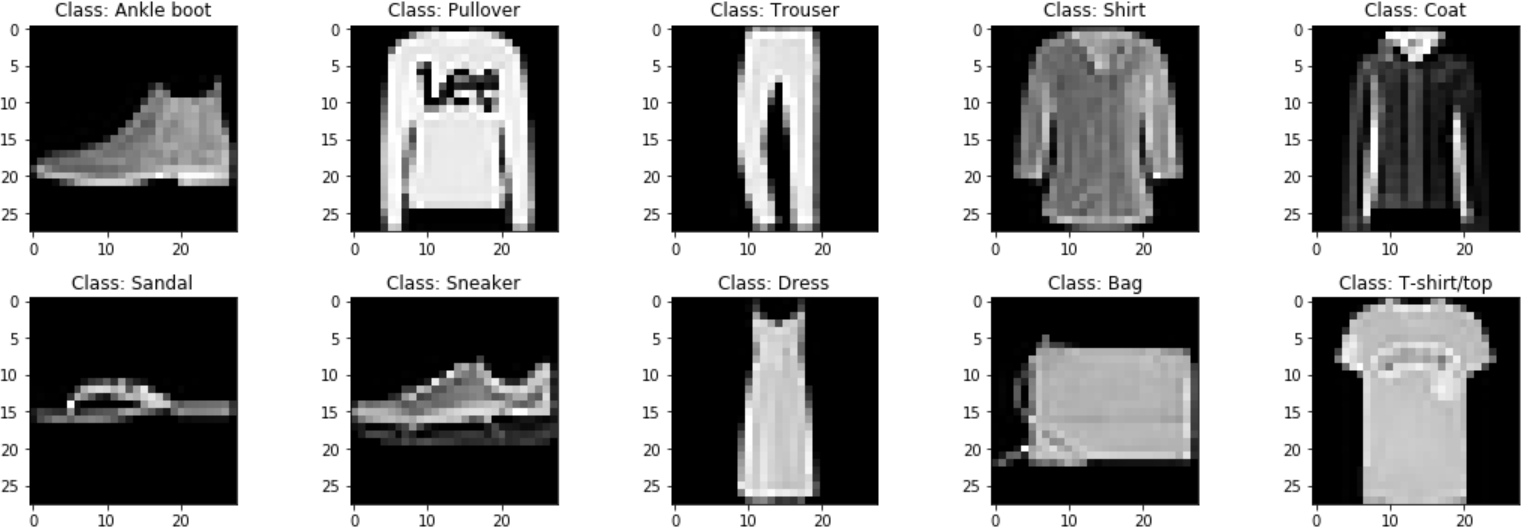
\includegraphics[width=0.6\textwidth]{Images/Examples_Fashion_MNIST.png}
% 	\end{center}
% \end{frame}

\begin{frame}{Communication-Efficient Learning of Deep Networks from Decentralized Data}
    by HB McMahan et al.
    \begin{itemize}
        \item Lays down the fundamentals concepts and algorithms of FL
        \item Focuses on algorithmic convergence and tries to minimize the number of GEs
        \item Does not take in consideration the latency of each GE
    \end{itemize}
    
\end{frame}


\begin{frame}{PipeFL: Hardware/Software co-Design of an FPGA Accelerator for Federated Learning}
    by Zixiao Wang et al.
    \begin{itemize}
        \item Integrated an FPGA-based accelerator in an open-source FL framework
        \item Fully focused on the data-center FL setting, using high-end FPGAs
        \item Generic architecture that can compute any model, but not optimized for any single one
        \item Compares only against a CPU implementation
    \end{itemize}%
\end{frame}

\begin{frame}{Unique Characteristics and Challenges of FL}
    FL literature has identified the following characteristics:
    
    System Heterogeneity
    
    Statistical Heterogeneity
    
    Expensive Communication
\end{frame}

\begin{frame}{System Heterogeneity}
    Clients can differ to each other in:\\
	\begin{itemize}
	    \item computational capabilities, hardware architecture \& resources
	    \item communication capabilities, reliability \& bandwidth
	\end{itemize}
	Consequences:\\
	\begin{itemize}
	    \item "stragglers" impede the entire process
	    \item random disconnections
	    \item unavailable clients
	\end{itemize}
\end{frame}

\begin{frame}{System Heterogeneity}
	\centering
	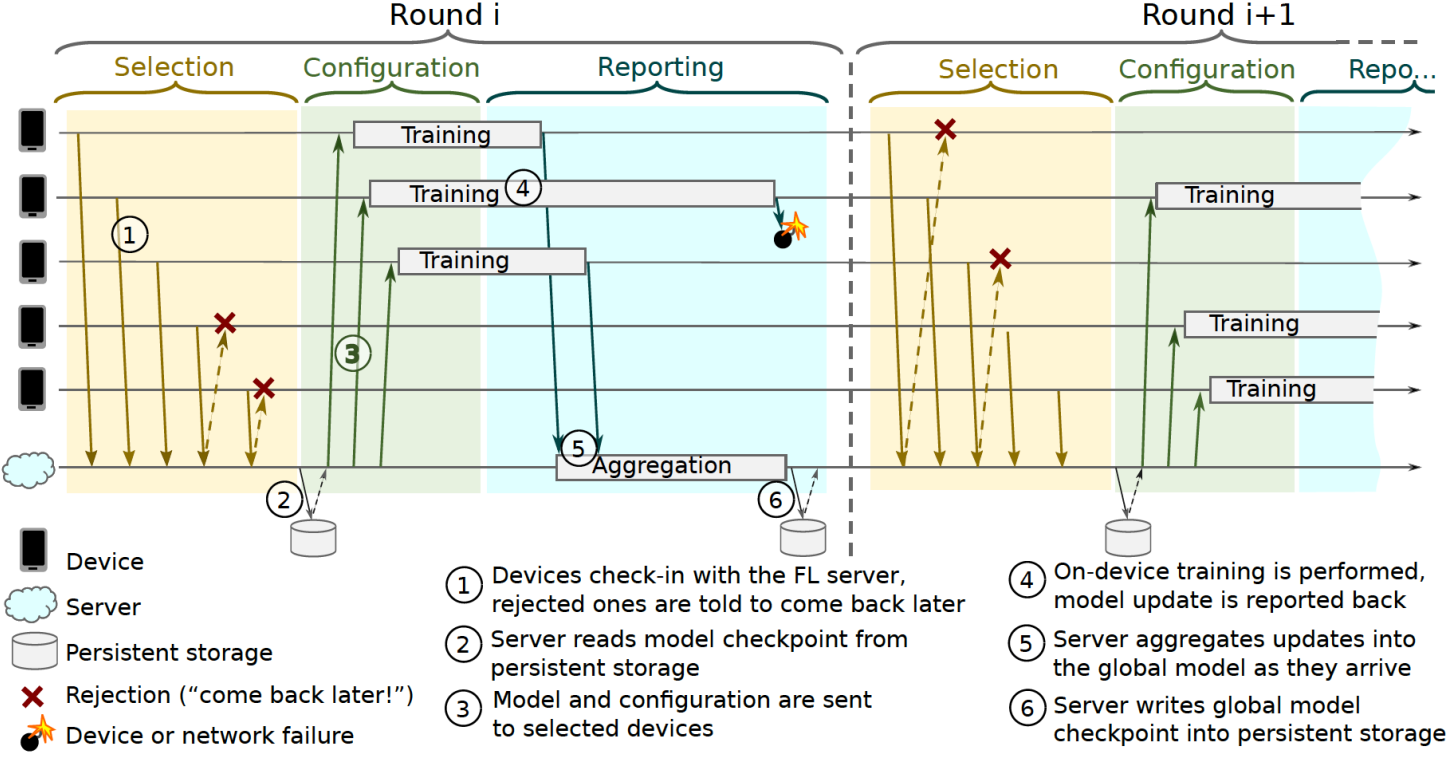
\includegraphics[height=0.75\textheight]{Images/Diagrams/fl_protocol.png}\\
\end{frame}

\begin{frame}{Statistical Heterogeneity}
    Independent and Identically Distributed (IID) dataset:\\
	\begin{itemize}
	    \item all examples have the same probability distribution
	    \item all examples are mutually independent
	\end{itemize}
    
    In practice, clients have data collection biases, thus non-IID datasets are more common.
    
    Huge ramifications in model convergence and overall training time!
\end{frame}

\begin{frame}{Statistical Heterogeneity}
	\begin{minipage}{0.45\textwidth}
        \begin{figure}[H]
            \centering
    		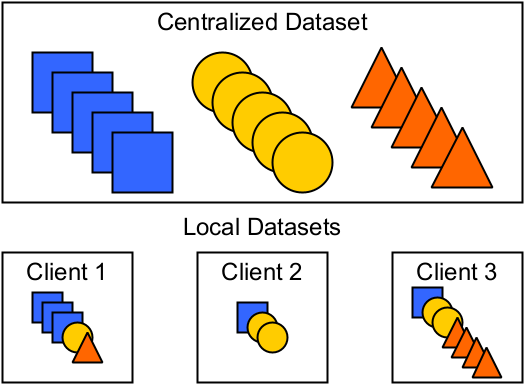
\includegraphics[width=1\textwidth]{Images/Diagrams/data_distribution.png}\\
    		\caption*{Centralized vs. Local Datasets}
    	 \end{figure}
	\end{minipage}%
	\begin{minipage}{0.6\textwidth}
		\hspace{0.35cm}Data distribution can be non-IID due to:
		\begin{itemize}
		    \item label distribution skew
		    \item concept drift
		    \item quantity skew
		    \item etc.
		\end{itemize}
	\end{minipage}%
\end{frame}

\begin{frame}{Expensive Communication}
Complete models are shared between the server and the clients -> large messages

edge devices usually have slow and unreliable connections

Communication is a critical bottleneck!
\end{frame}
